\chapter{Porównanie testowalności na przykładzie aplikacji}
\label{analiza_testow}

\section{Opis doświadczenia}
Doświadczenie polega na przeanalizowaniu przykładowej aplikacji dla Systemu Android zaprojektowanej na dwa sposoby. Wersja pierwsza to aplikacja napisana w standardowej architekturze, wersja druga to ten sam program napisany przy wykorzystaniu \textit{Clean Architecture}. Do tego celu zdecydowano się wykorzystać
aplikację \textit{JSON Web Token Authentication for Android} napisaną przez Victora Albertosa \cite{website:victor:aplication} , a której źródła udostępnione są w serwisie GitHub na licencji \textit{open source}.

W części doświadczalnej analizę ograniczono do testowalności w zakresie testów jednostkowych i wczesnych testów integracyjnych pomijając analizę na etapie testów systemowych czy akceptacyjnych z powodu braku dostępu do wymagań systemowych i wymagań klienta. Jednakże już na podstawie analizy testów jednostkowych i wstępnego testu integracyjnego można z dużym prawdopodobieństwem ocenić, czy zastosowanie TDD i architektury \textit{Clean Architecture} poprawi testowalność programu i spowoduje polepszenie testowalności również na dalszych etapach procesu testowego.

\section{Opis aplikacji}
\textit{JSON Web Token Authentication for Android} autentykuje użytkowników Androida i iOS korzystając z \textit{REST API} serwera \textit{Parse} oraz textit{JSON\footnote{JSON, JavaScript Object Notation – lekki format wymiany danych komputerowych. JSON jest formatem tekstowym, bazującym na podzbiorze języka JavaScript. Źródło: Wikipedia.} Web Tokens (JWT)}. JWT to otwarta, według standardu przemysłowego RFC 7519\cite{website:jwt:rfc7519}, metoda do uwierzytelniania stron w środowisku aplikacji internetowych. Wykorzystywana jest do przekazywania tożsamości użytkowników między dostawcą, a odbiorcą usług internetowych lub innego typu uwierzytelnień zgodnie z logiką biznesową. 

Serwer \textit{Parse} to wspólna platforma do przechowywania danych i interakcji z usługami internetowymi dla aplikacji mobilnych. Wielu programistów decyduje się na wykorzystanie tej platformy, zamiast pisać własne rozwiązania w tym zakresie.

Victor Albertos zdecydował się użyć wyżej wymienionego rozwiązania, aby zwiększyć pielęgnowalność swojej aplikacji: móc modyfikować logikę biznesową nie modyfikując aplikacji po stronie klienta. Serwer Parse, jako rozwiązanie uniwersalne, zapewniał takie podejście i wpisywał się doskonale w koncepcję autora aplikacji.

\section{Zasada działania}
Użytkownik loguje się za pomocą swojej nazwy użytkownika i hasła do serwera \textit{Parse}. Jeżeli nie posiada jeszcze konta na serwerze, może założyć je bezpośrednio z używanego programu. Jeżeli użytkownik istnieje, od chwili zalogowania może korzystać z dostępnych mu usług serwera, a logując się z wielu urządzeń korzysta z wielosesyjności systemu. 

\section{Analiza aplikacji pod względem testowalności}
W tej pracy autor skupia się na budowie aplikacji tylko z punktu widzenia testowania aplikacji, nie będzie więc analizowany szczegółowo kod programu. Przeprowadzone natomiast zostaną testym na podstawie których można w wystarczającej części ocenić, czy zmiana struktury oprogramowania na \textit{Clean Architecture} oraz zastosowanie  \textit{Test Driven Development} wpłynie pozytywnie na testowalność oprogramowania, w tym przypadku tej wybranej aplikacji.

\newpage
\subsection{Budowa analizowanej aplikacji napisanej w architekturze standardowej}
Schemat budowy aplikacji \textit{JSON Web Token Authentication for Android} zbudowanej w standardowej architekturze przedstawia się tak, jak to pokazano na rysunku \ref{fig:app_std}.

\begin{figure}[!htb]
    \centering
    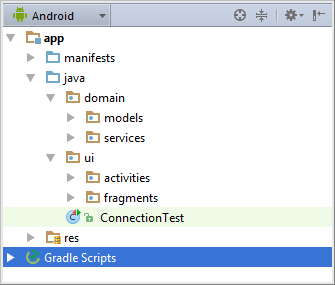
\includegraphics[width=10cm]{imgs/ch6_app_st.png}
    \caption
{Schemat budowy aplikacji w architekturze standardowej}
    \label{fig:app_std}
\end{figure} 

Aplikacja podzielona jest na warstwę domenową i warstwę interfejsu użytkownika. W celu przetestowania interfejsu użytkownika, utworzono jeden test, który w zależności od kontekstu można nazwać integracyjnym, systemowym, bądź nawet końcowym. Test polega na zalogowaniu się do programu za pomocą przykładowych danych i otrzymaniu wyniku, czy autentykacja przebiegła pomyślnie. Poza tym przypadkiem nie znaleziono żadnych innych testów, w tym jednostkowych. Z punktu widzenia programisty, można byłoby napisać je w każdym momencie. Jest to jednak trudne do wykonania z dwóch powodów: po pierwsze - ze względu na stopień uzależnienia warstwy domenowej i \textit{UI} od środowiska Android, a po drugie - programista piszący testy może (nawet nieświadomie) skupiać się na zapewnieniu pokrycia testami już gotowego kodu, zamiast na szukaniu błędów w programie. Do problemu tego nawiązano już w rozdziale \ref{opis_problemu}.

\subsection{Budowa analizowanej aplikacji wykorzystującej \textit{Clean Architecture}}
Każde z wymienionych w rozdziale \ref{propozycja_rozwiazania} podejść do uporządkowania architektury systemowej można wykorzystać do polepszenia testowalności aplikacji tworzonych dla systemu Android. Analizując opisywane rozwiązania krok po kroku można dojść do wniosku, że ich idea jest taka sama, a różnią się jedynie szczegółami. W tym wypadku autor \textit{JSON Web Token Authentication for Android} zdecydował się na \textit{The Clean Architecture}, zaprezentowaną w tej pracy w rozdziale \ref{clean_architecture_opis}.

\begin{figure}[!htb]
    \centering
    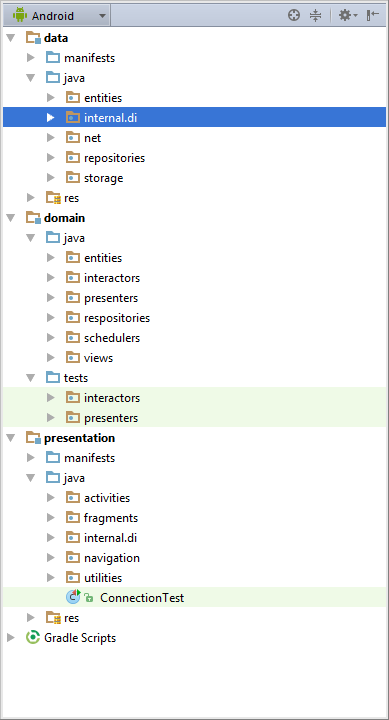
\includegraphics[width=10cm]{imgs/ch6_app_cl.png}
    \caption
{Schemat budowy aplikacji w \textit{Clean Architecture}}
    \label{fig:app_std}
\end{figure} 

Tym razem aplikacja została podzielona na trzy warstwy: zgodnie z nowym podejściem wydzielono warstwę przechowywania danych, za \textit{UI} odpowiada warstwa prezentacyjna, a warstwa domenowa została wzbogacona o dwa zestawy testów jednostkowych, które zostały napisane przed powstaniem kodu programu:
\begin{itemize}
\item
\textit{interactors} - \textit{opisać warstwę w domu}
\item
\textit{presenters} - \textit{opisać warstwę w domu},
\end{itemize}
Test interfejsu użytkownika pozostał ten sam, aczkolwiek jego zakres został ograniczony o przetestowane w testach jednostkowych zagadnienia. - \textit{sprawdzić w domu czy to prawda.}

\section{Przebieg doświadczenia}
Podczas doświadczenia przeprowadzono osobne pomiary dla obu projektów, wykorzystując to samo środowisko testowe (\textit{wziąć pojęcia ze słownika testerskiego}): Android Studio w wersji 1.5.1, ten sam komputer i ten sam emulator: Nexus\_5\_API\_23.

\section{Wyniki doświadczenia}
\label{wyniki_doswiadczenia}
\subsection{Architektura standardowa}
Wyniki doświadczenia dla aplikacji napisanej w architekturze standardowej przedstawiają się następująco:
\begin{itemize}
\item
Brak testów jednostkowych. Brak weryfikacji błędów w kodzie na bieżąco. Patrz rysunek \ref{fig:odwrocona_piramida}.

\begin{figure}[!htb]
    \centering
    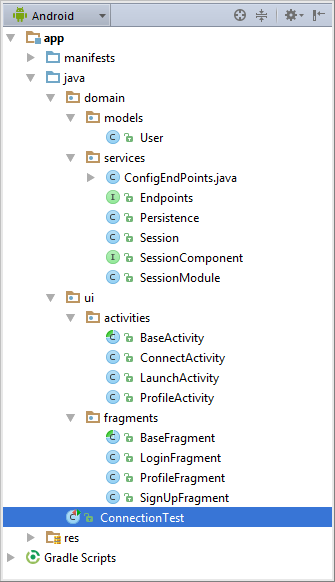
\includegraphics[width=10cm]{imgs/ch6_app_st_test1.png}
    \caption
{Brak testów jednostkowych. jedynym dostępnym jest test integracyjny.}
    \label{fig:app_std_test1}
\end{figure} 


\item
Jedynym testem jest \textit{ConnectionTest}. Czas trwania: 241s. Wymaga uruchomienia emulatora bądź podłączenia fizycznego urządzenia. W przypadku błędu w kodzie testy wydłużają się, gdyż za każdym razem trzeba uruchomić \textit{ConnectionTest}.
Wynik testu przedstawia rysunek \ref{fig:app_std_test2}

\begin{figure}[!htb]
    \centering
    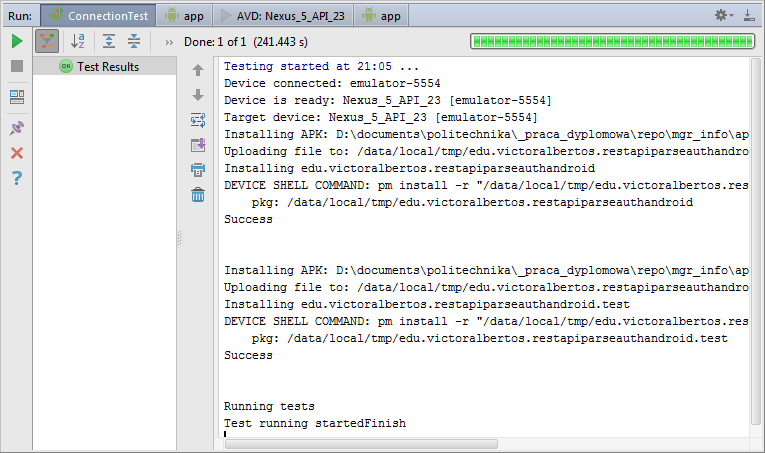
\includegraphics[width=15cm]{imgs/ch6_app_st_test2.png}
    \caption
{Wynik testu integracyjnego. Długi czas trwania.}
    \label{fig:app_std_test2}
\end{figure} 

\end{itemize}

\newpage
\subsection{\textit{Clean Architecture}}
\textit{---------draft-------------}

\begin{itemize}
\item
Tutaj są zarówno testy jednostkowe jak i test integracyjny \textit{ConnectionTest}.

Strukturę testów jednostkowych przedstawia rysunek \ref{fig:app_cl_test1}
\begin{figure}[!htb]
    \centering
    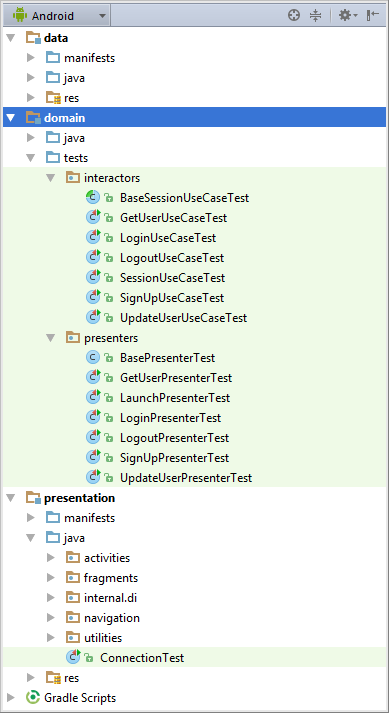
\includegraphics[width=10cm]{imgs/ch6_app_cl_test1.png}
    \caption
{Struktura testów jednostkowych}
    \label{fig:app_cl_test1}
\end{figure} 

\item
Wyniki testów jednostkowych przedstawiają rysunki \ref{fig:app_cl_test5}, \ref{fig:app_cl_test3} i \ref{fig:app_cl_test4}.

\begin{figure}[!htb]
    \centering
    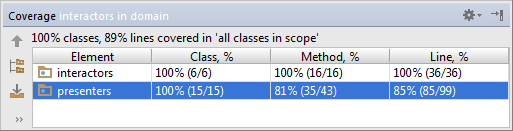
\includegraphics[width=12cm]{imgs/ch6_app_cl_test5.png}
    \caption
{Wyniki wraz z pokryciem kodu}
    \label{fig:app_cl_test5}
\end{figure} 

\begin{figure}[!htb]
    \centering
    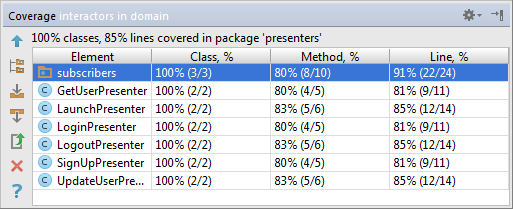
\includegraphics[width=12cm]{imgs/ch6_app_cl_test3.png}
    \caption
{Wyniki wraz z pokryciem kodu}
    \label{fig:app_cl_test3}
\end{figure} 

\begin{figure}[!htb]
    \centering
    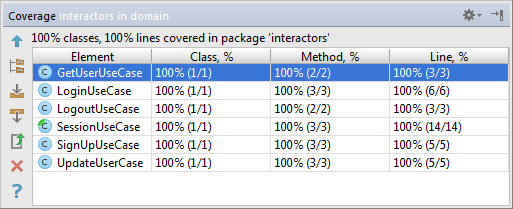
\includegraphics[width=12cm]{imgs/ch6_app_cl_test4.png}
    \caption
{Wyniki wraz z pokryciem kodu}
    \label{fig:app_cl_test4}
\end{figure} 

\item
Test integracyjny również jest szybszy i trwa 167s. Wynik przedstawiony na rysunku \ref{fig:app_cl_test6}

\begin{figure}[!htb]
    \centering
    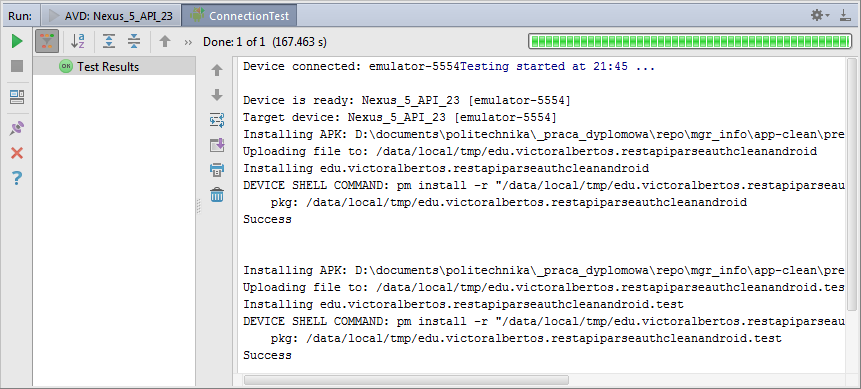
\includegraphics[width=15cm]{imgs/ch6_app_cl_test6.png}
    \caption
{Wynik testu integracyjnego}
    \label{fig:app_cl_test6}
\end{figure} 

\end{itemize}
